\section{Literature review}

\subsection{Related works}

\begin{frame}{Mathematical models: Compartmental}
    \begin{block}{\gls{SEIR} model \cite{brauerCompartmentalModelsEpidemiology2008}}
        \begin{equation*}
            \begin{aligned}
                S' &= - \beta(N)SI \\
                E' &= \beta(N)SI - \kappa E \\
                I' &= \kappa E - \alpha I \\
                R' &= f \alpha I \\
                N' &= - (1 - f) \alpha I
            \end{aligned}
        \end{equation*}
    \end{block}

    \begin{figure}
        \centering
        \begin{tikzpicture}[->, > = stealth', node distance = 2cm, thick]
            \node[state]               (S) {S};
            \node[state, right of = S] (E) {E};
            \node[state, right of = E] (I) {I};
            \node[state, right of = I] (R) {R};
            \draw (S) edge node[above]{$\beta$}  (E)
                (E) edge node[above]{$\kappa$} (I)
                (I) edge node[above]{$\alpha$} (R);
        \end{tikzpicture}
        \caption{States graph for the SEIR model}
        \label{fig:seir-model-transition-graph}
    \end{figure}
\end{frame}

\begin{frame}{Mathematical models: Agent-based}
    \begin{figure}[!htb]
        \centering
        \subcaptionbox{Transmission networks}{
            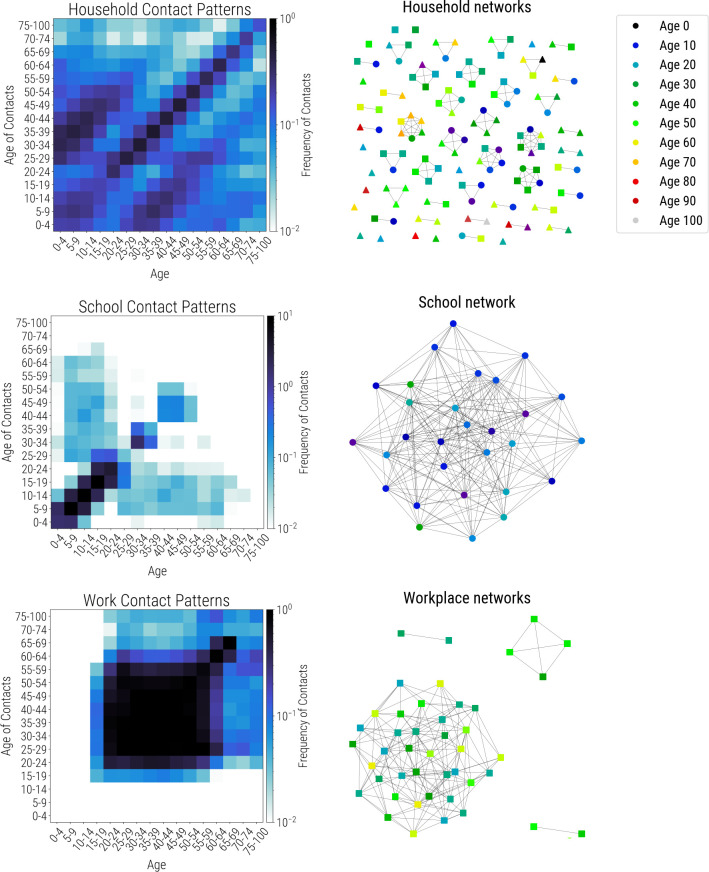
\includegraphics[scale=0.7]{covasim-networks.jpg}
        }
        \subcaptionbox{States graph}{
            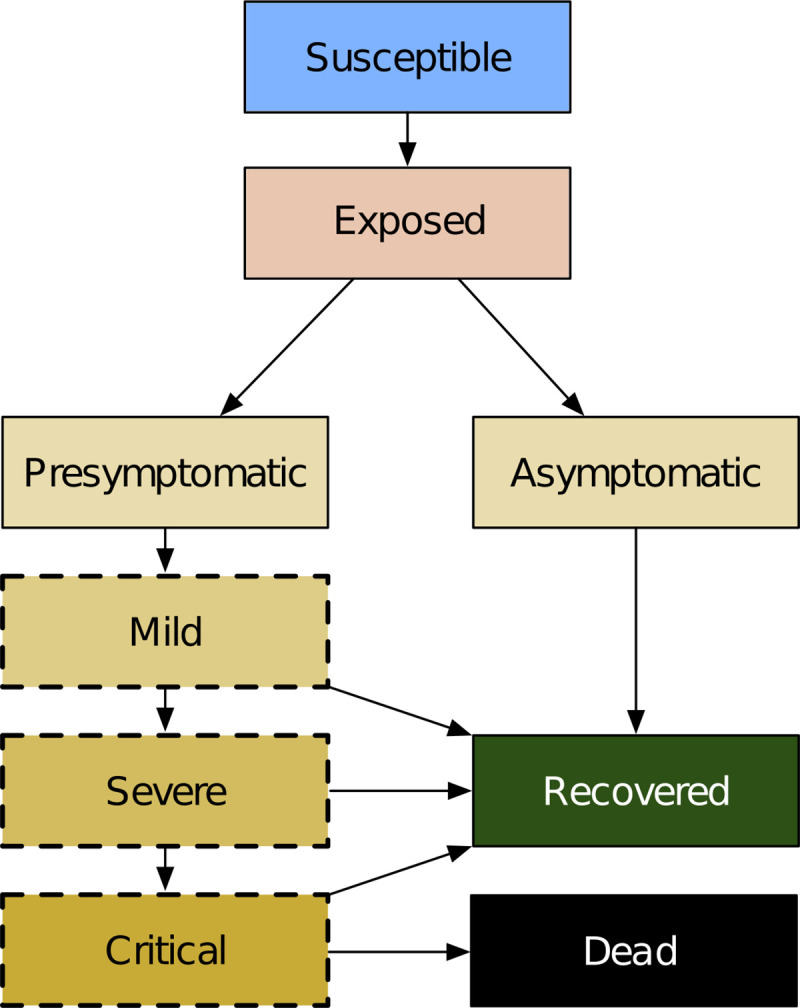
\includegraphics[scale=0.5]{covasim-compartments.jpg}
        }
        \caption{Covasim model \cite{kerrCovasimAgentbasedModel2021}}
        \label{fig:covasim-schematics}
    \end{figure}
\end{frame}

% \begin{frame}{Mathematical models: Covid-19}
%     Changes made to classical compartmental model for infectious disease \cite{zhaoModelingEpidemicDynamics2020,heSEIRModelingCOVID192020,ndairouMathematicalModelingCOVID192020,bastosModelingForecastingEarly2020,sarkarModelingForecastingCOVID192020}:
%     \begin{itemize}
%         \item<2-> Inclusion of compartments that represent government interventions
%         \item<3-> Inclusion of compartments that specifically represent the behavior of SARS-NCOV-2
%         \item<4-> Separation of the infectious compartment into multiple compartments representing the severity of the patients
%     \end{itemize}
% \end{frame}

\begin{frame}{Mathematical models: Pros \& cons}
    \begin{exampleblock}<1->{Pros}
    \begin{itemize}
        \item Explainable
        \item Based on many years of research
        \item Easy to understand and implement
    \end{itemize}
    \end{exampleblock}

    \begin{alertblock}<2->{Cons}
    \begin{itemize}
        \item Low representational capabilities
        \item The represented dynamics are stationary
        \item Unrealistic assumptions about real-world scenarios
    \end{itemize}
    \end{alertblock}
\end{frame}

\begin{frame}{Data-driven models}
    \begin{itemize}
        \item<1-> \gls{ARIMA} models \cite{ceylanEstimationCOVID19Prevalence2020,singhPredictionCOVID19Pandemic2020,ribeiroShorttermForecastingCOVID192020}
        \item<2-> Explainable \gls{ANN} encoder \cite{ramchandaniDeepCOVIDNetInterpretableDeep2020}
        \item<3-> \glspl{RNN} \cite{chimmulaTimeSeriesForecasting2020,shahidPredictionsCOVID19Deep2020}
        \begin{itemize}
            \item \glspl{LSTM}
            \item \glspl{Bi-LSTM}
            \item \glspl{GRU}
        \end{itemize}
    \end{itemize}
\end{frame}

\begin{frame}{Data-driven models: Pros \& cons}
    \begin{exampleblock}<1->{Pros}
    \begin{itemize}
        \item High prediction accuracy
        \item Allow for modeling without needing domain knowledge
    \end{itemize}
    \end{exampleblock}

    \begin{alertblock}<2->{Cons}
    \begin{itemize}
        \item Unexplainable
        \item Relied on large amount of data
        \item Inability to capture the true disease dynamics
    \end{itemize}
    \end{alertblock}
\end{frame}

\begin{frame}{Novel compartmental models: Using mobility data}
    \begin{figure}[!htb]
        \centering
        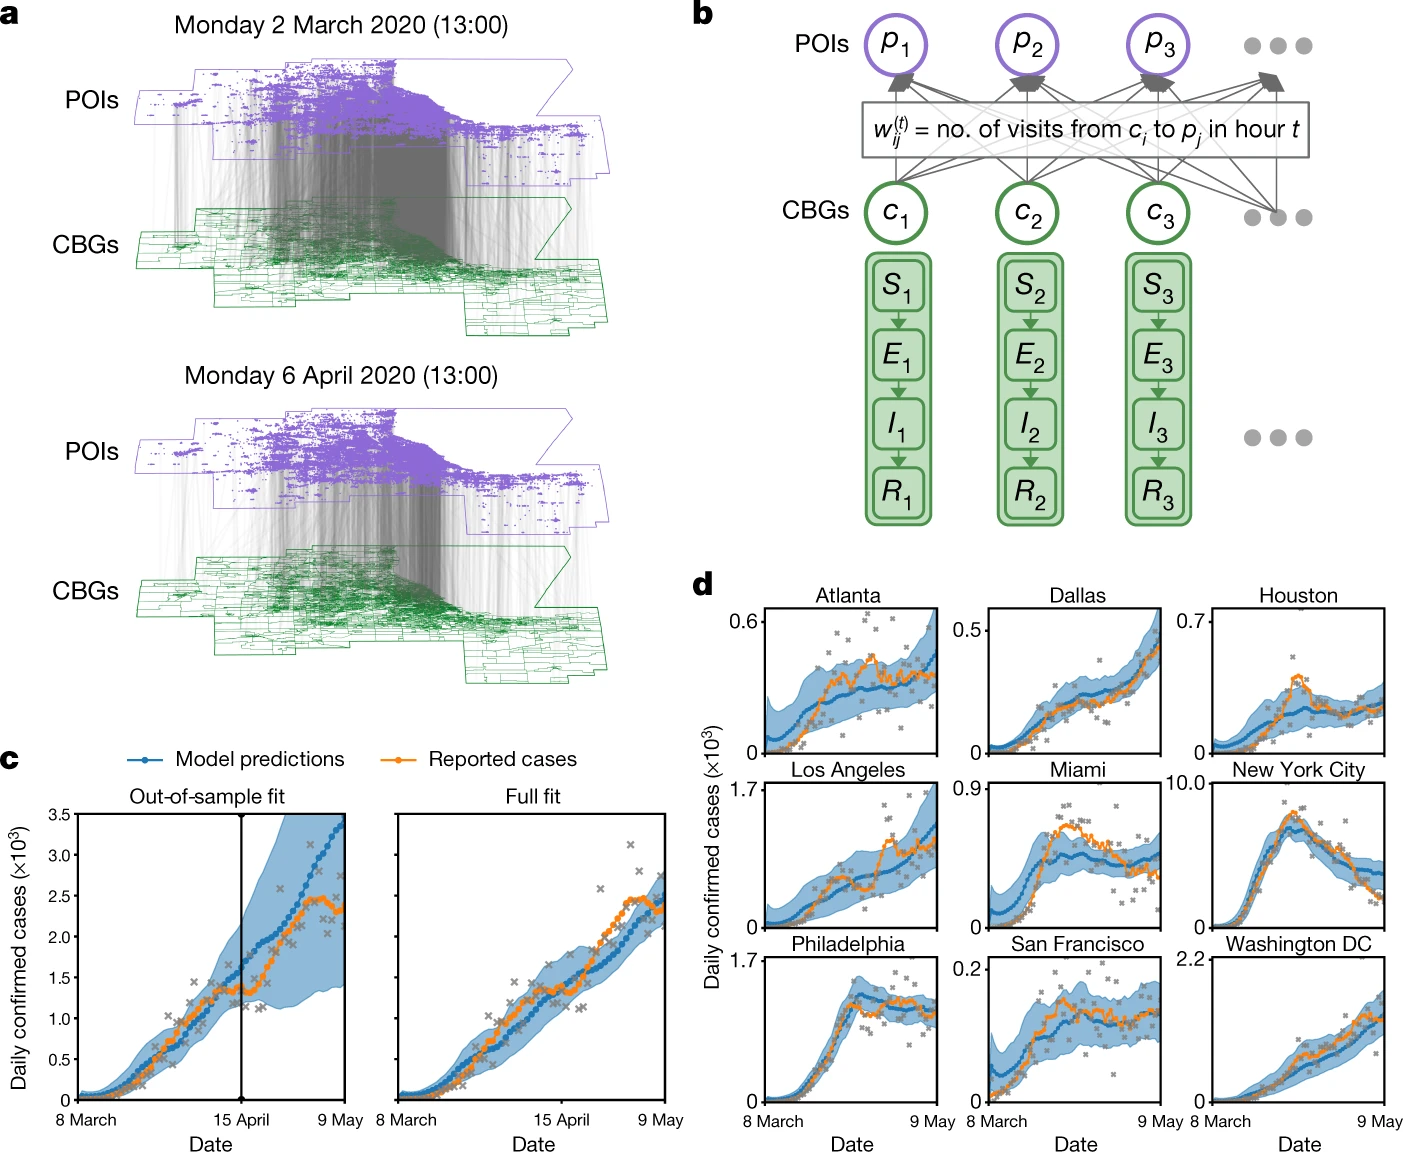
\includegraphics[scale=0.2]{nature-chang-mobility-covid19.png}
        \caption{SEIR model informed with mobility data \cite{changMobilityNetworkModels2021}}
        \label{fig:nature-chang-mobility-covid19}
    \end{figure}
\end{frame}

\begin{frame}{Novel compartmental models: Using ANNs}
    \begin{figure}[!htb]
        \centering
        \subcaptionbox{QSIR \cite{dandekarMachineLearningAidedGlobal2020a}}{
            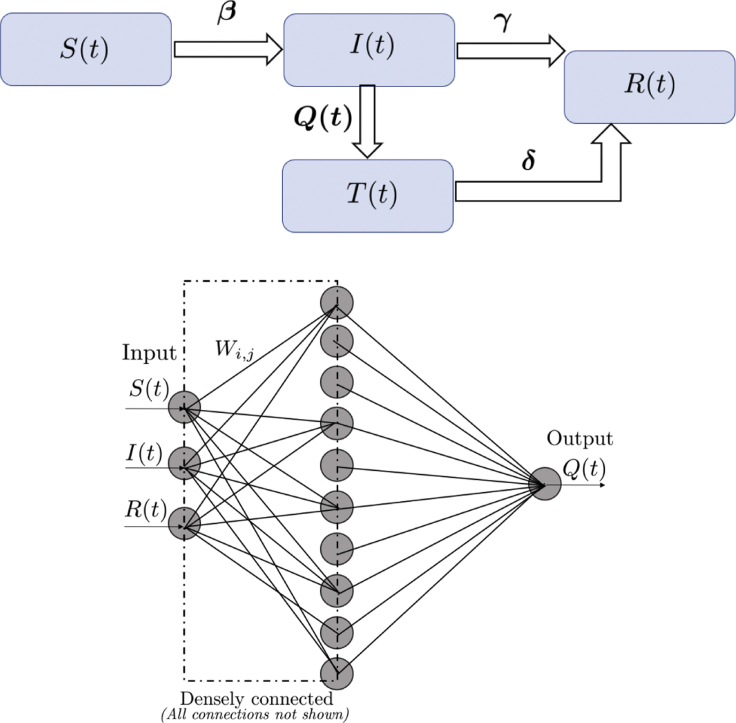
\includegraphics[width=0.4\linewidth]{mit-dandekar-qsir.jpg}
        }
        \subcaptionbox{Time-dependent SIR \cite{jungRealWorldImplicationsRapidly2020}}{
            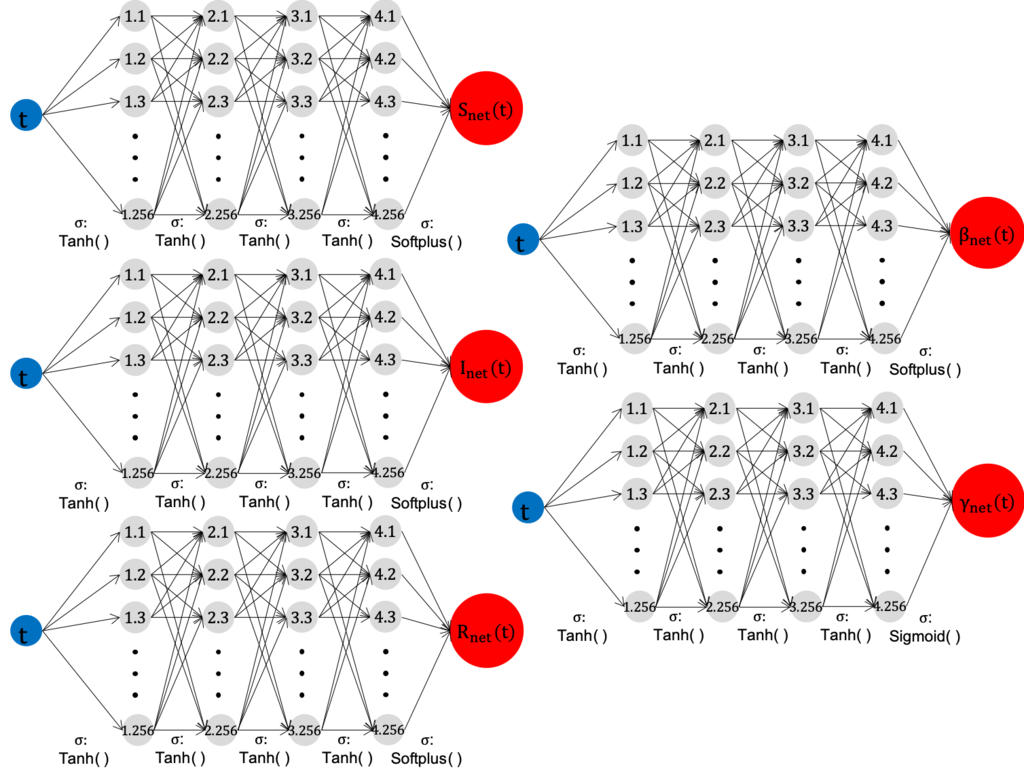
\includegraphics[width=0.4\linewidth]{jung-sir-pinn.png}
        }
        \caption{Predict the parameters of compartmental models with \glspl{ANN}}
        \label{fig:compartmentals-models-with-neural-networks}
    \end{figure}
\end{frame}

\subsection{Artificial neural networks}

\begin{frame}[fragile]{Multi-layer perceptron: Graph representation}
    \begin{figure}[h]
        \centering
        \begin{neuralnetwork}
            \newcommand{\nodex}[2]{$x_#2$}
            \newcommand{\nodey}[2]{$y_#2$}

            \inputlayer[count=3, bias=false, title={}, text=\nodex]
            \hiddenlayer[count=4, bias=false, title={}]
            \linklayers[title=$W_1$]
            \hiddenlayer[count=4, bias=false, title={}]
            \linklayers[title=$W_2$]
            \outputlayer[count=2, bias=false, title={}, text=\nodey]
            \linklayers[title=$W_3$]
        \end{neuralnetwork}
        \caption{A multi-layer perceptron with four layers}
        \label{fig:multi-layer-perceptron}
    \end{figure}
\end{frame}

\begin{frame}{Multi-layer perceptron: Mathematical representation}
    \begin{block}<1->{Multi-layer perception}
        \begin{equation*}
            g(X) = \phi_n(W_n \phi_{n - 1}(\cdots (W_2 \phi_1(W_1 X + b_1) + b_2) + \cdots) + b_n)
        \end{equation*}
    \end{block}

    \begin{theorem}<2->
        Given appropriate weights, \glspl{ANN} can approximate any arbitrary function $f: \mathbb{R}^M \to \mathbb{R}^N$ \cite{cybenkotApproximationSuperpositionsSigmoidal, hornikApproximationCapabilitiesMultilayer1991, hornikMultilayerFeedforwardNetworks1989}
    \end{theorem}
\end{frame}

\begin{frame}[fragile]{Training neural networks: Back-propagation}
    \begin{block}{\gls{MSE}}
        \begin{equation*}
            \mathcal{L} = \frac{1}{N} \sum_{i=1}^N (g(X_i) - Y_i)^2
        \end{equation*}
    \end{block}
    \begin{figure}[h]
        \centering
        \scalebox{0.6}{
            \begin{neuralnetwork}
                \newcommand{\nodex}[2]{$x_#2$}
                \newcommand{\nodey}[2]{$y_#2$}

                \inputlayer[count=3, bias=false, title={Input\\layer}, text=\nodex]
                \hiddenlayer[count=4, bias=false, title={Hidden\\layer}]
                \linklayers[title=$\frac{\delta \mathcal{L}}{\delta a^1}\frac{\delta a^1}{\delta z^1}$,style={<-,draw=red}]
                \hiddenlayer[count=4, bias=false, title={Hidden\\layer}]
                \linklayers[title=$\frac{\delta \mathcal{L}}{\delta a^2}\frac{\delta a^2}{\delta z^2}$,style={<-,draw=red}]
                \outputlayer[count=2, bias=false, title={Output\\layer}, text=\nodey]
                \linklayers[title=$\frac{\delta \mathcal{L}}{\delta a^3}\frac{\delta a^3}{\delta z^3}$,style={<-,draw=red}]
            \end{neuralnetwork}
        }
        \caption{Graph representation of the back-propagation algorithm}
        \label{fig:multi-layer-perceptron-backpropagation}
    \end{figure}
\end{frame}

\begin{frame}{Physics-informed neural networks}
    \begin{figure}[h]
        \centering
        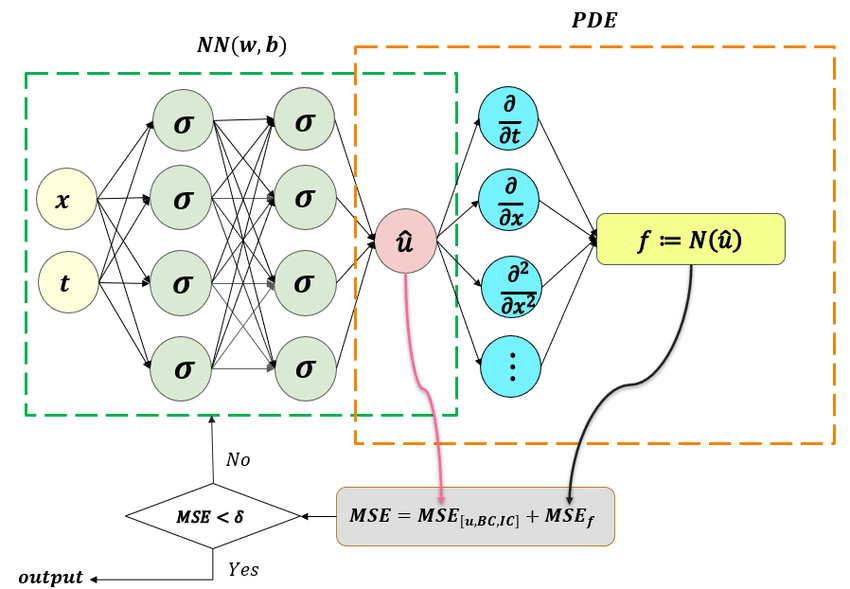
\includegraphics[scale=0.3]{pinn-schematic.png}
        \caption{The schematic of PINNs for solving PDEs \cite{guoSolvingPartialDifferential2020}.}
        \label{fig:pinn-schematic}
    \end{figure}
\end{frame}

\begin{frame}[fragile]{Neural ordinary differential equations: Idea}
    \begin{columns}
        \begin{column}{0.5\linewidth}
            \begin{figure}[h]
                \centering
                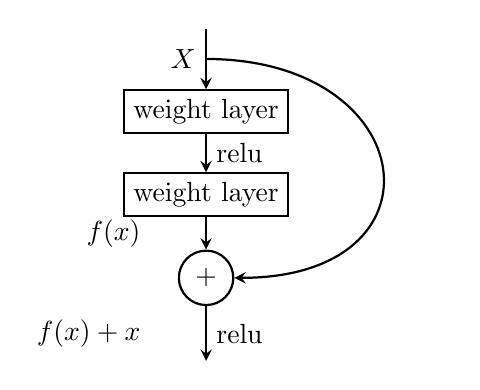
\begin{tikzpicture}[->, >=stealth, node distance = 3em, thick]
                    \tikzset{
                        block/.style  = {draw, thick, rectangle},
                        arith/.style  = {draw, thick, circle},
                        input/.style  = {coordinate},
                        output/.style = {coordinate}
                    }
                    \node[input] (IN) {};
                    \node[block, below of = IN] (W1) {weight layer};
                    \node[block, below of = W1] (W2) {weight layer};
                    \node[arith, below of = W2] (ADD) {+};
                    \node[output, below of = ADD] (OUT) {+};

                    \draw[->] (IN) to node[left, name = X]{$X$} (W1);
                    \draw[->] (X) to [out = 0, in = 0, looseness = 2.5] (ADD);
                    \draw[->] (W1) to node[right]{relu} (W2);
                    \draw[->] (W2) to node[xshift = -2em, left]{$f(x)$} (ADD);
                    \draw[->] (ADD) to node[xshift = -2em, left]{$f(x) + x$} node[right]{relu} (OUT);
                \end{tikzpicture}
                \caption{Skip connection}
                \label{fig:residual-network-skip-connection}
            \end{figure}
        \end{column}
        \begin{column}{0.5\linewidth}
            \begin{block}<1->{Euler method}
                \begin{equation*}
                    h_{t+1} = h_t + f(h_t, \theta_t)
                \end{equation*}
                \begin{equation*}
                    \frac{dh(t)}{dt} = f(h(t), t, \theta).
                \end{equation*}
            \end{block}
        \end{column}
    \end{columns}
\end{frame}

\begin{frame}{Neural ordinary differential equations: Formulation}

    \begin{block}<1->{NeuralODE output and loss}
        \begin{equation*}
            L(z(t_1)) = L\left(z(t_0) + \int_{t_0}^{t_1}{f(z(t), t, \theta)dt}\right)
        \end{equation*}
    \end{block}

    \begin{itemize}
        \item<2-> Memory efficiency
        \item<2-> Adaptive computation
        \item<2-> Scalable and invertible normalizing flows
        \item<2-> Continuous time series models
    \end{itemize}
\end{frame}

\begin{frame}{Neural ordinary differential equations: Outputs}
    \begin{figure}[h]
        \centering
        \subcaptionbox{ResNet}{
            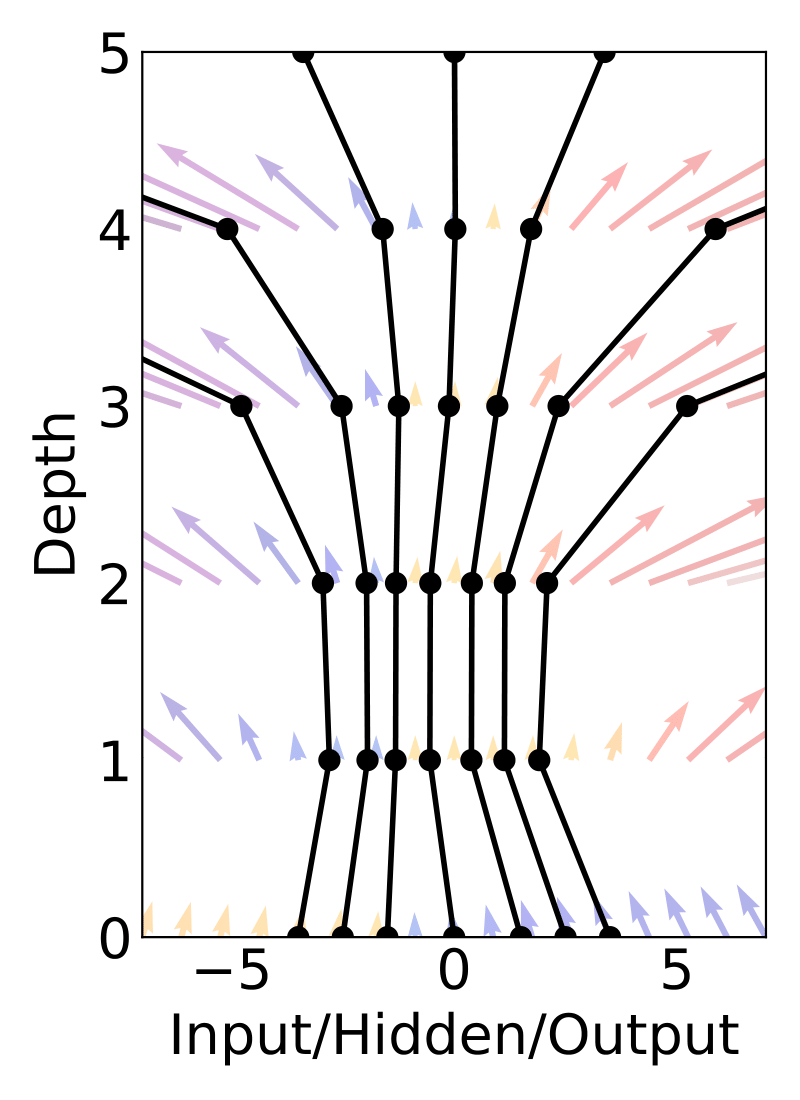
\includegraphics[scale=0.1]{neuralode_resnet.png}
        }
        \subcaptionbox{NeuralODE}{
            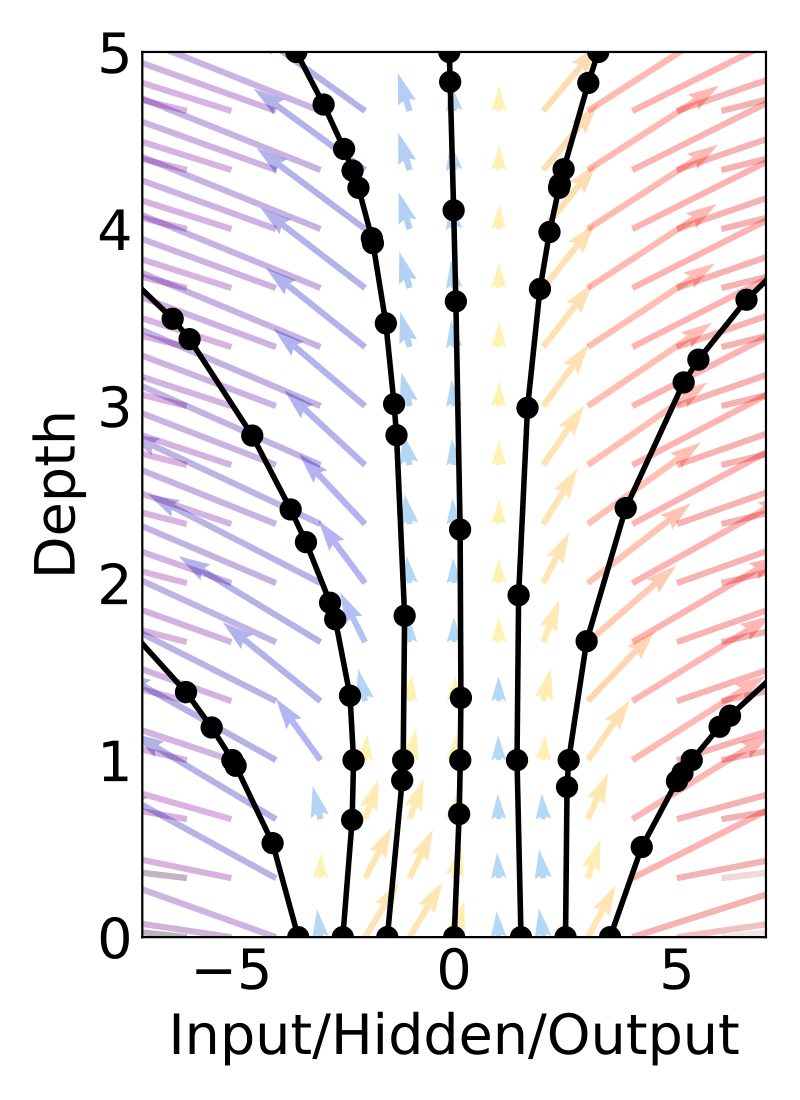
\includegraphics[scale=0.1]{neuralode_odenet.png}
        }
        \caption{Comparison between ResNet's discrete state transformations and NeuralODE continuous state transformations}
        \label{fig:resnet-vs-odenet}
    \end{figure}
\end{frame}

\begin{frame}{Neural ordinary differential equations: Gradients}
    \begin{figure}[h]
        \centering
        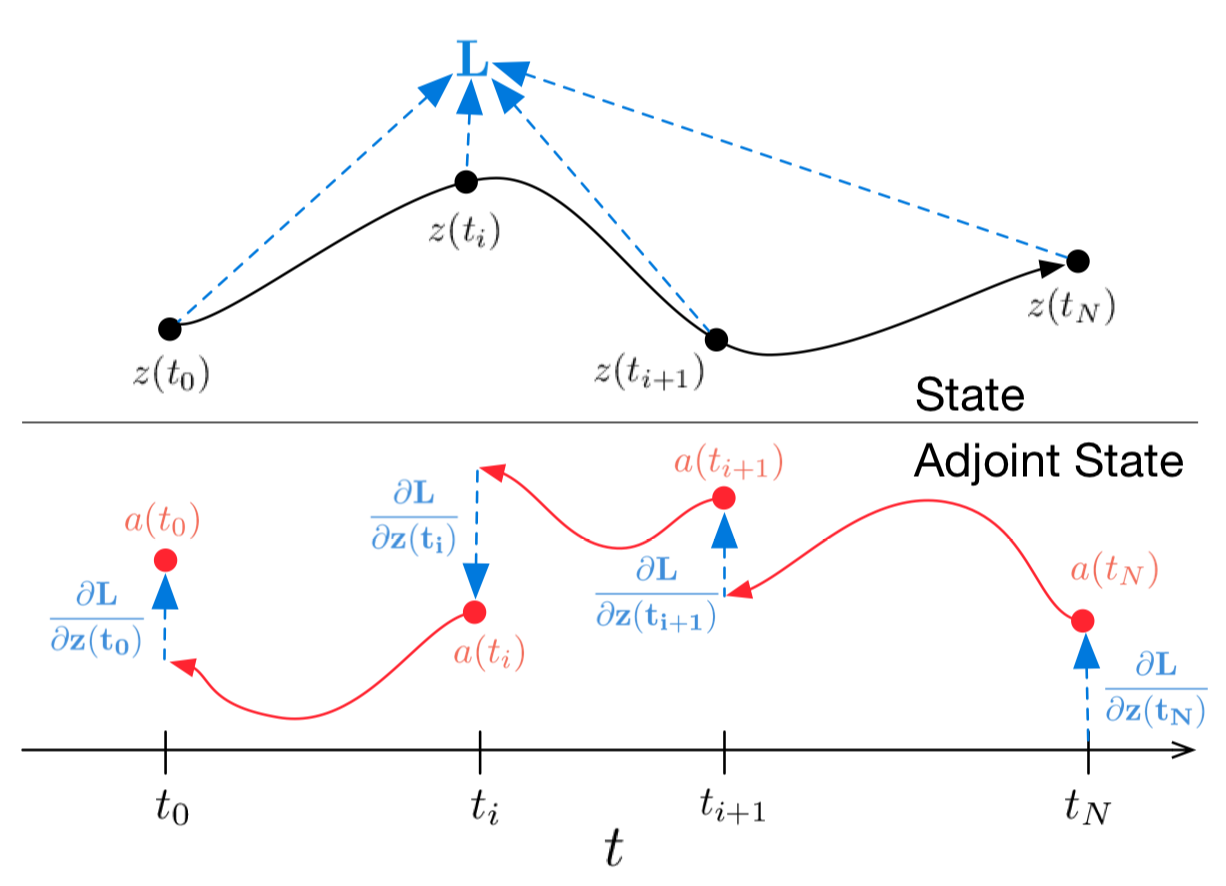
\includegraphics[scale=0.4]{neuralode-adjoint.png}
        \caption{Reverse-mode differentiation of an ODE solution. \cite{chenNeuralOrdinaryDifferential2019}}
        \label{fig:neuralode-adjoint}
    \end{figure}
\end{frame}
